\section{Experiments and Analysis}
\subsection{Evaluation framework and metrics}
Đánh giá trả lời ba câu hỏi: \textbf{RQ1}, transcript hạn chế suy luận vị trí đến đâu trong mô hình đã khai báo;
\textbf{RQ2}, đáp án dịch vụ còn hữu ích đến đâu; và \textbf{RQ3}, đánh đổi đó cần bao nhiêu truy vấn/dữ liệu.
Cận lý thuyết không phụ thuộc vào một attacker học cụ thể; benchmark chỉ kiểm tra các attacker hữu hạn trên workload này.

\begin{tabularx}{\linewidth}{@{}P{.8cm}P{4.1cm}Y@{}}\toprule
\textbf{Case} & \textbf{Target} & \textbf{Quan sát thực sự dùng trong trial chính}\\\midrule
S1 & GPS tại tick đang xét & Một packet tại tick dịch vụ công khai; không xem trước/sau.\\
S2 & Proxy tọa độ cửa sổ muộn & Tất cả wire trong 540--600 s; target là trung bình bốn GPS ticks. Chưa đo suy luận nơi dừng ngữ nghĩa.\\
S3 & Đường đã đi & Toàn wire 0--600 s; tái dựng 31 GPS theo timestamp, rồi gộp sai số.\\
S9 & GPS đầu phiên & Toàn wire, biết public clock và mốc bắt đầu.\\
S10 & GPS cuối phiên & Toàn wire, biết phiên đóng tại 600 s; không giả định attacker không biết lúc kết thúc.\\\bottomrule
\end{tabularx}

Với target $x_i$, ước lượng $\hat x_i$ và sai số Euclid theo mét $e_i=\|x_i-\hat x_i\|$:
\[
\operatorname{Hit100}=\frac1N\sum_{i=1}^N\mathbf1\{e_i\le100\},\qquad
\operatorname{MAE}=\frac1N\sum_{i=1}^Ne_i.
\]
Hit100 thấp hơn và MAE cao hơn có lợi cho privacy trong \emph{cùng task/attacker protocol}. Hai phép đo bổ sung:
Hit100 thể hiện xác suất định vị trong vùng thực dụng, MAE thể hiện độ lệch trung bình; một số sai số rất lớn
có thể làm MAE cao dù Hit100 vẫn cao. Chúng không chứng minh formal privacy hay anonymity.

\textbf{Utility theo đáp án.} Reference $T_{t,\psi}$ là tối đa năm POI đúng theo GPS và purpose; danh sách client
trả về là toàn bộ kết quả phù hợp đã sắp xếp, không bị cắt ở năm. Recall@5 là
$|T_{t,\psi}\cap U_t|/|T_{t,\psi}|$, với $U_t$ là tập ứng viên hợp lệ thực nhận; nhờ cùng bộ lọc/total order,+nó cũng là độ phủ reference top-five sau local ranking. Reference rỗng là N/A và được ghi mẫu số.
Macro là trung bình đều bốn purposes có reference hợp lệ: gần nhất theo khoảng cách, nhanh nhất theo cost
di chuyển, trong bán kính 1.000 m và ít vòng đường nhất đối với một đích local đã biết.

Gộp tick trong trip, các trip/draw trong family, rồi trung bình family. TEST có 20 family; mỗi family hai
chuyến và ba defense draws. Bootstrap \textbf{10.000 lần theo family}, giữ ghép cùng family giữa các phương pháp,
seed công khai 20261028. CI là percentile 95\%; không coi 120 trip-draw là 120 family độc lập.
Hit và MAE dùng model được chọn riêng theo loss; hai số trong một ô không nhất thiết từ cùng một estimator.

\textbf{Vì sao cần bộ đo này?} (i) Target và cửa sổ quan sát vẫn có cùng ý nghĩa khi output là một điểm hoặc
nhiều điểm; (ii) utility đo đáp án thực nhận thay vì chỉ độ lệch điểm giả; (iii) request/response tính đủ các
fake events; (iv) metrics gốc được giữ khi áp dụng được. Bộ đo là một \emph{protocol kết hợp metrics đã biết},
không tuyên bố phát minh MAE/Recall hay thay thế mọi phép đo của nghiên cứu trước.

S4--S6 không có score thực nghiệm chính: hệ quả Bayes ở Phần~\ref{sec:privacy} có điều kiện trên kênh target.
S7 phân biệt request payload không gửi với intent tương quan route; S8 cần quan hệ đồng hành và dữ liệu
liên người riêng. N/A không đồng nghĩa đã bảo vệ hoặc đã thất bại.

\clearpage
\subsection{Dataset construction and environment}
Workload dùng mạng đường có hướng SUMO, các phiên di chuyển native và catalogue POI công khai trong
repository. Mỗi phiên giữ tọa độ/trạng thái đường, timestamp và reference POI riêng để đánh giá. Các ràng buộc
scenario xác định \emph{target/cửa sổ suy luận}; không lựa chọn lại tuyến theo điểm privacy của mô hình.
Các family gom những chuyến liên quan để tránh rò rỉ giữa TRAIN và TEST do cùng cấu trúc nguồn.
Nguồn \texttt{cache\_fresh\_native\_20261012\_v2} được sinh bằng SUMO bước 1 s trên mạng native đã lưu:
đề xuất các cặp nhánh đường có đích cách ít nhất 600 m, giới hạn tuyến 4 km, kiểm tra overlap edge-set
và cân bằng tốc độ công khai 6/8 m/s giữa các split. Lọc eligibility dựa trên geometry/calibration công khai,
không đọc score defense. Trial hiện tại dùng hai phiên ngày 7/8 của mỗi family, giữ cửa sổ 600 s và stop cuối;
không sinh cohort mới hoặc sửa sample. Source generator và hashes đi kèm artifact nguồn.

\begin{tabularx}{\linewidth}{@{}P{4.2cm}Y@{}}\toprule
\textbf{Thành phần} & \textbf{Thiết lập}\\\midrule
Nguồn và không gian & Cùng native graph của cohort đã đóng băng; 66.189 trạng thái đường và 418 POI. Tọa độ quy đổi sang mét nhất quán.\\
Chia family & 48 family: 20 TRAIN / 8 SELECTION / 20 TEST, không giao family giữa các split.\\
Số chuyến/draw & Hai chuyến/family; một draw ở TRAIN/SELECTION, ba draws ở TEST: 176 trip-draw/arm, trong đó 120 TEST.\\
Thời gian & Mỗi chuyến 0--600 s, 31 target ticks cách 20 s. Fake-query có thêm packet theo lịch tự nhiên.\\
Dịch vụ & Mỗi tọa độ truy vấn mọi category với L60; cùng catalogue, reference, local ranking và tie-break.\\
Cache & Current: packet hiện tại; epoch60: tích lũy trong đoạn 60 s; session: tích lũy cả phiên, là chế độ chính. Metadata tĩnh.\\
Môi trường & Python 3.12, NumPy 2.4.6, SciPy 1.17.1, scikit-learn 1.7.1; OPENBLAS/OMP một thread. Nền tảng chi tiết được lưu trong protocol.\\\bottomrule
\end{tabularx}

Reference được tính trên cùng provider đầy đủ; mỗi purpose dùng cost/filter tương ứng và cùng total order.
Đích cần cho minimum-detour chỉ nằm trong workload local; nó không được gửi như payload thật.
GPS dùng đánh giá local ở mỗi target tick không phải một lần đọc mới được đưa vào lớp bảo vệ Geo-I.
Số lần private read và số lần local ranking vì vậy khác nhau.

Đây là \textbf{controlled comparison trên cohort đã xem}, không phải xác nhận trên tuyến/thành phố mới.
Family split phục vụ fit/chọn attacker; cấu trúc bản đồ và workload đã được dùng trong quá trình phát triển.
Catalogue nhỏ, đáp án tĩnh và session cache có thể làm Recall gần bão hòa; không suy rộng sang catalogue rất lớn,
POI hết hạn hoặc dịch vụ cá nhân hóa chưa được mô hình hóa.

\subsection{Comparison methods and protocol}
\begin{tabularx}{\linewidth}{@{}P{3.4cm}P{3.6cm}Y@{}}\toprule
\textbf{Phương pháp} & \textbf{Output} & \textbf{Cấu hình và fidelity}\\\midrule
Raw GPS & Một GPS thật / tick & Control không bảo vệ, kiểm tra target có thể quan sát được.\\
Geo-I/REM Z (K1) & Một Z / tick & Phát lại anchors đã lưu của cùng proposed run; không lấy mẫu REM mới.\\
TransProtect* & Một tọa độ thay thế & Candidate K10, tám TRAIN targets, $\alpha_{\rm TP}=10000$, $\varepsilon=0{,}005$ m$^{-1}$; Markov thay predictor neural gốc.\\
Semantic correlation* & GPS thật + bốn dummy & K5, pool128; semantic từ POI công khai, predictor thực nghiệm thay AMap/LSTM.\\
Fake-query insertion* & Tập real/dummy + fake packets & K5; tối đa hai fake giữa lần thật, chờ 5--15 s, 24 ứng viên, similarity 0,75; road/history adaptation.\\
\textbf{GeoI-BQ v1} & Năm Q-only / tick & Phát lại đúng Q/time của cấu hình chính đã đóng băng, không tạo draws mới.\\\bottomrule
\end{tabularx}
\textbf{Dấu * luôn nghĩa adaptation}, không là implementation chính thức hoặc kết quả do tác giả paper báo cáo.
Giữ những cơ chế có thể audit; thay predictor/data được công bố rõ. Không ép các epsilon hoặc K khác bản chất
thành ``cùng mức privacy''. AnotherMe offline và DLS/RDG lịch sử không là đối chứng online gần đây.

\textbf{Attacker bank.} Cùng họ geometry/history, \textbf{ExtraTrees (64 trees)}, \textbf{kNN-1/kNN-5} và prior;
endpoint thêm ordered/geometry-linked sequences. Fit trên TRAIN, chọn riêng từng method/scenario/loss trên
SELECTION bằng mean+SE cho MAE hoặc mean$-$SE cho Hit, rồi đánh giá TEST. Đây là attacker kiểm thử của ta,
không phải tuyên bố lấy nguyên attacker của paper. Feature API chỉ nhận coordinates/timestamps;
không nhận Z nội bộ của proposed, belief, cờ real/fake, khóa hay chỉ mục evaluator.
Public clock đã biết nên fake timing không được xem là bí mật. S3 tái dựng tại đúng timestamp GPS;
fake packets bổ sung vẫn ở trong observation window và cost.

\clearpage
\subsection{Main results}
\subsubsection{Privacy theo scenario}
Mỗi ô là \textbf{Hit100 (\%) / MAE (m)}; chiều tốt cho bảo vệ là Hit thấp, MAE cao.
Các con số là trung bình family TEST. CI đầy đủ ở Phụ lục A.
\begin{small}\par\smallskip\noindent\begin{tabularx}{\linewidth}{@{}P{3.1cm}XXXXX@{}}\toprule
\textbf{Phương pháp} & \textbf{S1} & \textbf{S2} & \textbf{S3} & \textbf{S9} & \textbf{S10} \\
\midrule
Raw GPS & 100{,}000 / 0{,}0 & 100{,}000 / 0{,}0 & 100{,}000 / 0{,}0 & 100{,}000 / 0{,}0 & 100{,}000 / 0{,}0 \\
Geo-I/REM Z (K1) & 18{,}522 / 338{,}5 & 37{,}500 / 214{,}3 & 18{,}522 / 338{,}5 & 5{,}833 / 435{,}8 & 35{,}000 / 246{,}8 \\
TransProtect* & 82{,}984 / 54{,}4 & 94{,}167 / 28{,}7 & 82{,}984 / 54{,}4 & 96{,}667 / 17{,}8 & 90{,}833 / 33{,}6 \\
Semantic correlation* & 82{,}258 / 41{,}9 & 100{,}000 / 8{,}2 & 82{,}258 / 41{,}9 & 100{,}000 / 5{,}3 & 100{,}000 / 7{,}3 \\
Fake-query insertion* & 53{,}387 / 1213{,}0 & 92{,}500 / 239{,}1 & 98{,}790 / 13{,}3 & 99{,}167 / 42{,}2 & 100{,}000 / 6{,}4 \\
\textbf{GeoI-BQ v1} & 0{,}188 / 2104{,}6 & 0{,}000 / 2124{,}2 & 0{,}188 / 2104{,}6 & 0{,}000 / 1986{,}4 & 0{,}000 / 2124{,}2 \\
\bottomrule\end{tabularx}\par\smallskip
\end{small}

Raw khôi phục các target với Hit100 100\% và sai số gần 0, xác nhận phép đo không che những target trực tiếp
quan sát được. GeoI-BQ có Hit100 0--0,188\% và MAE khoảng 1,99--2,12 km; REM-Z trực tiếp còn Hit100
5,833--37,500\%. Trong bank này, công bố Q-only từ thư viện public rộng giúp hạn chế định vị hơn công bố Z.
Đây là \emph{quan sát thực nghiệm}; cận formal ở Phần 3 không được suy ra từ MAE cao.

Ba adaptation có utility rất cao nhưng target vẫn dễ định vị hơn. Fake-query thể hiện đặc biệt rõ việc phải
đọc cả hai metrics: S1 có MAE 1.213 m nhưng Hit100 vẫn 53,387\%; khi nối cả cửa sổ S3 và biết public clock,
Hit100 lên 98,790\%. Packet giả bổ sung không tự bảo đảm indistinguishability khi timing thật có thể nhận diện.
Không suy từ kết quả adaptation rằng mọi bản triển khai gốc của paper đều có nhược điểm với cùng mức độ.

S2 chỉ là proxy tọa độ cuối cửa sổ; S9/S10 biết mốc đầu/cuối. Không gọi các số này là đã xác nhận stop semantics,
identity người/xe hoặc prediction tương lai. S1 và S3 có thể bằng nhau khi selection chọn cùng kiểu estimator;
không vì vậy mà hai threat có cùng ý nghĩa.

\subsubsection{Utility theo từng purpose và CI}
Session cache; mọi giá trị là Recall@5 (\%), app vẫn trả toàn danh sách phù hợp.
\begin{small}\par\smallskip\noindent\begin{tabularx}{\linewidth}{@{}P{3.9cm}XXXXX@{}}\toprule
\textbf{Phương pháp} & \textbf{Trung bình} & \textbf{Gần nhất} & \textbf{Nhanh nhất} & \textbf{Bán kính} & \textbf{Ít vòng đường} \\
\midrule
Raw GPS & 99{,}999 & 100{,}000 & 100{,}000 & 100{,}000 & 99{,}995 \\
Geo-I/REM Z (K1) & 99{,}700 & 99{,}753 & 99{,}753 & 99{,}625 & 99{,}668 \\
TransProtect* & 99{,}996 & 100{,}000 & 100{,}000 & 100{,}000 & 99{,}986 \\
Semantic correlation* & 99{,}999 & 100{,}000 & 100{,}000 & 100{,}000 & 99{,}997 \\
Fake-query insertion* & 99{,}999 & 100{,}000 & 100{,}000 & 100{,}000 & 99{,}997 \\
\textbf{GeoI-BQ v1} & 99{,}595 & 99{,}638 & 99{,}641 & 99{,}388 & 99{,}712 \\
\bottomrule\end{tabularx}\par\smallskip
\end{small}
GeoI-BQ đạt \textbf{\PrimaryRecall\%}, CI95\% macro \PrimaryCI\%.
So với ba adaptation, macro giảm khoảng 0,4 điểm phần trăm. Đây là trade-off có dấu âm, không gọi là
vượt đối chứng về utility. Radius là purpose nhạy hơn vì catalogue ứng viên phải chứa các POI đủ gần GPS thật.
Các phép đo gần 100\% cũng phản ánh workload nhỏ và cache tĩnh; không dùng chúng để khẳng định mọi
query purpose trong ứng dụng thực đều đã được bao phủ.
\par\smallskip\noindent\begin{tabularx}{\linewidth}{@{}P{4.5cm}XXX@{}}\toprule
\textbf{Đối chứng} & \textbf{Recall (\%)} & \textbf{BQ trừ đối chứng (pp)} & \textbf{CI95\% (pp)} \\
\midrule
Raw GPS & 99{,}999 & -0{,}404 & [-0{,}775; -0{,}095] \\
Geo-I/REM Z (K1) & 99{,}700 & -0{,}105 & [-0{,}542; 0{,}275] \\
TransProtect* & 99{,}996 & -0{,}401 & [-0{,}773; -0{,}093] \\
Semantic correlation* & 99{,}999 & -0{,}404 & [-0{,}775; -0{,}096] \\
Fake-query insertion* & 99{,}999 & -0{,}404 & [-0{,}775; -0{,}096] \\
\bottomrule\end{tabularx}\par\smallskip

CI tuyệt đối từng purpose và chênh lệch theo tất cả controls được giữ trong Phụ lục B;
không chỉ chọn so sánh có lợi.

\clearpage
\subsubsection{Đánh đổi privacy--utility--cost}
\begin{center}
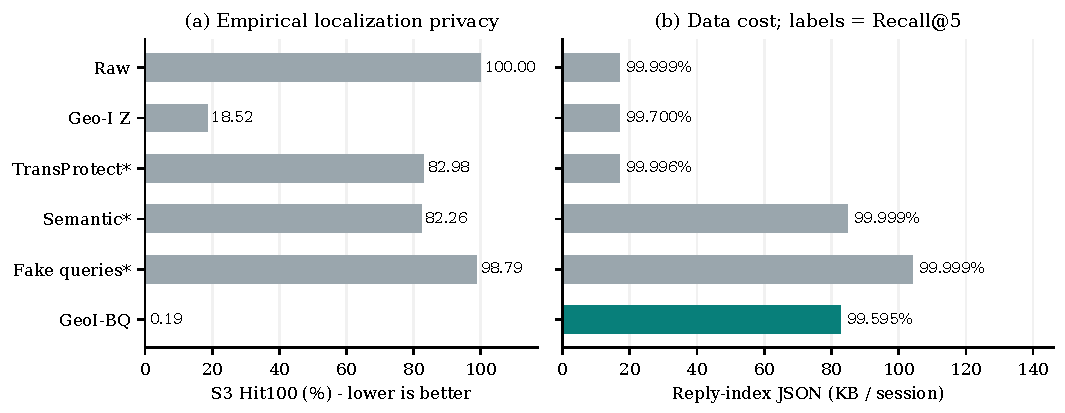
\includegraphics[width=\linewidth]{figures/tradeoff.pdf}
\captionof{figure}{So sánh trên cùng cohort. Trái: S3 Hit100 thấp hơn có lợi cho privacy. Phải: reply-index JSON KB/phiên;
nhãn là session Recall@5. Đồ thị thể hiện ba mặt của đánh đổi, không gộp thành một score tùy ý. Dấu * chỉ adaptation.}
\label{fig:tradeoff}
\end{center}
\par\smallskip\noindent\begin{tabularx}{\linewidth}{@{}P{3.6cm}XXXXX@{}}\toprule
\textbf{Phương pháp} & \textbf{Packet} & \textbf{Query điểm} & \textbf{Request KB} & \textbf{Reply KB} & \textbf{Sinh / tick ms} \\
\midrule
Raw GPS & 31{,}00 & 31{,}00 & 5{,}846 & 16{,}843 & <0{,}001 \\
Geo-I/REM Z (K1) & 31{,}00 & 31{,}00 & 6{,}352 & 16{,}921 & -- \\
TransProtect* & 31{,}00 & 31{,}00 & 6{,}351 & 16{,}847 & 3{,}287 \\
Semantic correlation* & 31{,}00 & 155{,}00 & 31{,}754 & 84{,}770 & 0{,}993 \\
Fake-query insertion* & 38{,}04 & 190{,}21 & 39{,}418 & 104{,}033 & 0{,}759 \\
\textbf{GeoI-BQ v1} & 31{,}00 & 155{,}00 & 31{,}756 & 82{,}557 & -- \\
\bottomrule\end{tabularx}\par\smallskip

Trung bình mỗi phiên 600 s; KB = 1.000 byte. ``Query điểm'' đếm từng tọa độ, gồm mọi category theo cùng
provider API. Fake-query gửi trung bình 38,04 packets thay vì 31; mọi packet phụ đều được tính.
GeoI-BQ dùng 155 point queries, cùng mức K5 như Semantic* nhưng nhiều hơn singleton Z/TransProtect*.
Chi phí này giúp lấy ứng viên đủ rộng mà không gửi nhu cầu thật.

``Sinh/tick'' là tổng thời gian sinh adapter mới chia 31 input ticks; không là p95 hay latency end-to-end.
GeoI-BQ và REM-Z được replay từ outputs cũ nên không có generation timing đồng bộ trong trial này (ký hiệu --).
Service replay dùng shared warm cache và thứ tự chạy; không dùng nó để tuyên bố phương pháp nào nhanh hơn.
Byte chỉ gồm request/reply-index JSON, chưa gồm metadata POI đầy đủ, HTTP/TLS, mạng hay năng lượng thiết bị.

\clearpage
\subsubsection{Metrics gốc: giữ đúng hợp đồng}
\par\smallskip\noindent\begin{tabularx}{\linewidth}{@{}P{3.7cm}XXXXX@{}}\toprule
\textbf{Phương pháp} & \textbf{EIE S3 (m)} & \textbf{$\Delta c$ (m)} & \textbf{ASR} & \textbf{DER} & \textbf{Path count} \\
\midrule
Raw GPS & 0{,}0 & 0{,}00 & N/A & N/A & N/A \\
Geo-I/REM Z (K1) & 338{,}5 & 688{,}65 & N/A & N/A & N/A \\
TransProtect* & 54{,}4 & 47{,}44 & N/A & N/A & N/A \\
Semantic correlation* & 41{,}9 & N/A & N/A & N/A & N/A \\
Fake-query insertion* & 13{,}3 & N/A & N/A & N/A & N/A \\
\textbf{GeoI-BQ v1} & 2104{,}6 & N/A & N/A & N/A & N/A \\
\bottomrule\end{tabularx}\par\smallskip

EIE cho point estimator ở S3 chính là MAE, không tạo thêm một kết quả độc lập. Với output singleton,
Eq.13 travel-cost distortion của TransProtect được đo bằng
\[
\Delta c=\sum_{d}\pi(d)\,|c(x,d)-c(y,d)|,
\]
với tám đích/prior chọn từ TRAIN, directed shortest-path metres và quy ước disconnected của provider.
Đây là \textbf{local-target proxy}: TransProtect* khoảng 47,44 m, REM-Z khoảng 688,65 m; không phải parity
với thí nghiệm Rome/SF gốc. Q-only hoặc real+dummy không có một released singleton $y$ duy nhất,
nên Eq.13 là N/A; không lấy centroid hoặc chọn Q gần GPS thật để tạo số.

ASR cần posterior calibrated trên real-member theo định nghĩa paper; DER cần hàm similarity và threshold
tương ứng; indistinguishable-path count cần bộ kiểm tra path đúng contract nguồn. Hiện chưa đủ đầu vào
để tính các metric này một cách đối chiếu được, vì vậy giữ N/A kèm lý do thay vì đổi tên Hit100 thành ASR.

\subsection{Supporting analysis}
\textbf{Cache theo cùng provider tĩnh.} Bảng dưới dùng chính trial mới, giữ đủ sáu phương pháp.
Epoch60 tương ứng bộ nhớ từ đầu đoạn hiện tại; session tích lũy từ đầu chuyến.
\par\smallskip\noindent\begin{tabularx}{\linewidth}{@{}P{4cm}XXX@{}}\toprule
\textbf{Phương pháp} & \textbf{Current (\%)} & \textbf{Epoch60 (\%)} & \textbf{Session (\%)} \\
\midrule
Raw GPS & 99{,}999 & 99{,}999 & 99{,}999 \\
Geo-I/REM Z (K1) & 98{,}610 & 98{,}610 & 99{,}700 \\
TransProtect* & 99{,}996 & 99{,}996 & 99{,}996 \\
Semantic correlation* & 99{,}999 & 99{,}999 & 99{,}999 \\
Fake-query insertion* & 99{,}999 & 99{,}999 & 99{,}999 \\
\textbf{GeoI-BQ v1} & 96{,}780 & 97{,}123 & 99{,}595 \\
\bottomrule\end{tabularx}\par\smallskip

Cache giúp coverage tại GPS đang xét khi tập ứng viên hợp lệ lớn hơn. Nó không bảo đảm Recall tăng theo
thời gian người dùng di chuyển, và không tự suy ra metadata vẫn đúng khi giờ mở cửa/giá/trạng thái thay đổi.

\textbf{Response depth và GPS local.} Cấu hình hiện tại dùng L60 mỗi loại/Q. Reference local ở grid 20 s
đo chất lượng mà người dùng thực sự nhận được; protected GPS vẫn được pacing 60 s và cap riêng.
Không tính local ranking là một lần phát GPS mới. Thử nghiệm L30 trên cùng Q và ablation nội bộ ngày
14/10 chỉ được giữ ở Phụ lục C; chúng không đứng thay cho so sánh paper ở bảng chính.

\textbf{Tính bất biến và kiểm chứng.} Protocol/source pins được chốt trước generation đối chứng;
không thay defense sau TEST. Mỗi arm hoàn tất 120/120 TEST, không failure. Nếu có failure,
privacy thiếu coverage là N/A, utility không giao được là 0. Các tests bao phủ split không giao family, prefix không phụ thuộc
tương lai, stripping nhãn riêng khỏi feature API, cửa sổ cùng thời gian, cache causal và tính đủ fake events.
Verifier độc lập tái tính 392.832 ô utility, 600 family-level privacy scores và 528 native-cost trip values;
kiểm tra 5.456 proposed prefixes và đếm 104.168 point queries trên toàn 176 trip-draws mỗi arm.
Sửa metadata request công khai
L30 thành L60 phản ánh đúng provider thực tế của nguồn cũ; Q/time, POI masks, utility và độ dài bytes không đổi.
Chi tiết và source hashes được giữ ở Phụ lục D và artifact; kết quả cũ không bị ghi đè.

\textbf{Phạm vi kết luận.} Cùng cohort, source adapters và finite bank làm phép so sánh có thể kiểm tra;
chúng không giải quyết mọi khác biệt fidelity, không xác nhận generalization ngoài thành phố và không
thay thế formal guarantee. So sánh chính cho thấy GeoI-BQ có privacy thực nghiệm tốt trong bank đang xét,
utility rất cao nhưng thấp hơn các adaptation, và cost lớn hơn phương pháp singleton.
